\section{Introduction: basic concepts}

\label{intro}

The \textbf{goal} of this USER GUIDE is to specify how to use the \href{https://github.com/Unike267/Containers/pkgs/container/containers\%2Fimpl-arty}{ghcr.io/unike267/ containers/impl-arty:latest} container.

\subsection{Container: ghcr.io/unike267/containers/impl-arty:latest}

The \href{https://github.com/Unike267/Containers/pkgs/container/containers\%2Fimpl-arty}{ghcr.io/unike267/containers/impl-arty:latest} \cite{gh:container-implarty} is a container composed by several FLOS (Free/Libre and/or Open Source) tools to generate bitstreams for the Xilinx FPGAs Arty A7 35T and 100T from VHDL code.
These FLOS tools are:

\begin{itemize}
    \item GHDL \cite{gh:ghdl}
    \item GHDL Yosys Plugin \cite{gh:ghdl-plugin}
    \item Yosys \cite{gh:yosys} 
    \item Nextpnr-Xilinx \cite{gh:nextpnr-x}
    \item Project X-Ray \cite{gh:prjxray}
\end{itemize}

\noindent In this context, the workflow to generate a bitstream from VHDL code is as follows:

\begin{itemize}
    \item First, GHDL tool compiles the VHDL code of the design.
    \item Second, ghdl-yosys-plugin imports the synthesized code to Yosys. 
\footnote{This plugin is necessary because Yosys, by default, is designed to synthesize verilog.} 
\footnote{ghdl-yosys-plugin is a thin layer that converts the internal representation of \mintinline[breaklines]{bash}{--synth} to Yosys’ C API.}
    \item Then, Yosys synthesis suite performs the synthesis/mapping for Xilinx 7-Series FPGAs.
    \item Third, Nextpnr-Xilinx tool performs the P\&R specifically for the Arty A7 35T or 100T FPGA.
    \item Finally, Project X-Ray generates the bitstream.
\end{itemize}

\noindent In addition to this, openFPGALoader \cite{gh:openFPGALoader} is used to load the output bitstream into the Arty FPGAs, see section \ref{ofl}.

\vspace{5mm}

\noindent You can visualize the container workflow in figure \ref{fig:workf}. 

\begin{figure}[H]
    \centering
    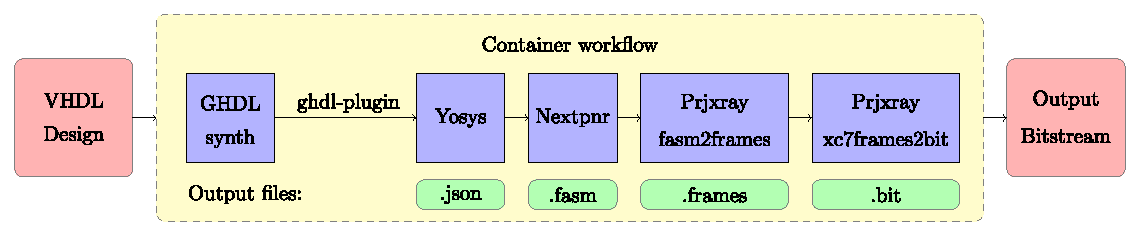
\includegraphics[width=151mm]{figures/container_workflow.pdf}
    \caption{Container workflow to generate bitstream from VHDL code.}
    \label{fig:workf}
\end{figure}

\subsection{Shell/Bash script}

\label{shell:script}

This container has the necessary FLOS tools installed inside it to generate bitstreams from your VHDL code. 
However, to automate the bitstream generation process, you can generate a shell/bash script \textit{(.sh)}.
This script will be executed inside the container and will perform all the steps to generate the bitstream using the internal FLOS tools installed in it.

\vspace{5mm}

\noindent The point is to facilitate the use of the container, in this order with a single command you will open a container from the downloaded image, run the shell/bash script inside this container, generate the bitstream from the VHDL sources and close the container simplifying the execution of the workflow.
In the section \ref{run} is specify how this script looks like.

\vspace{5mm}

\noindent To generate the bitstream from your VHDL code you must consider the relative paths that the shell/bash script points. 
In this context, if you run the container in the directory where your sources are, you must refers in the description of the script this paths.
More specifically, the part of the shell/bash code whose compile the VHDL code with GHDL must have the correct paths to include the sources and perform the compilation correctly.

\vspace{5mm}

\noindent To execute the sheel/bash script through the container you must add the argument \ref{cod:1} to open a shell inside it and execute your script. 
With this command you can execute several commands inside the open terminal by concatenating them through \textit{\&\&} symbol. 
For example, if you want to set a environment variable and then execute your script you can run \say{\mintinline[breaklines]{bash}{EnvVariable=YOUR_envVARIABLE && ./your_bash_script.sh}}.

\begin{code}
%\begin{minted}[frame=lines,framesep=2mm,baselinestretch=1.2,fontsize=\footnotesize,breaklines,linenos]{bash}
\begin{minted}[frame=lines,framesep=2mm,baselinestretch=1.2,fontsize=\footnotesize,breaklines]{bash}
                            sh -c "task1 && task2 && ..."
\end{minted}
\caption{Argument to add to the run container command to open a terminal inside it.}
\label{cod:1}
\end{code}

\vspace{5mm}

\noindent In conclusion, in order to operate in an easy and simplified way with the container you will open it, execute the workflow through the shell/bash script to generate the bitstream from your VHDL code and immediately close the container, all the execution through a single command \ref{cod:3}.
Instead of opening the container, locating you inside it and execute the workflow point by point.

\subsubsection{Shebang}

\label{shebang}

The shebang is a piece of code that indicates the path of the program that will interpret the script.
In this case, the interpreter is going to be bash.
Therefore, at the beginning of the script, you will indicate it through the piece of code \ref{cod:2}.

\vspace{10mm}

\begin{code}
\begin{minted}[frame=lines,framesep=2mm,baselinestretch=1.2,fontsize=\footnotesize,breaklines]{bash}
                                #!/usr/bin/env bash
\end{minted}
\caption{Shebang to interpret the script with bash.}
\label{cod:2}
\end{code}


\subsection{Container management tool}

In order to management the containers you must have a tool. 
Principally, there are two tools to perform this management: Podman \cite{podman} \cite{gh:podman} and Docker \cite{docker} \cite{gh:docker} \cite{gh:moby}.

\vspace{5mm}

\noindent In this case Podman is used, but for the Docker case it is basically the same.
First, you are going to download/install the tool aplliying the following commands depending your Linux distro:

\begin{itemize}
\item Fedora: \mintinline[breaklines]{bash}{sudo dnf -y install podman}
\item Debian: \mintinline[breaklines]{bash}{sudo apt-get -y install podman}
\item Arch Linux \& Manjaro Linux: \mintinline[breaklines]{bash}{sudo pacman -S podman}
\item Gentoo: \mintinline[breaklines]{bash}{sudo emerge app-containers/podman}
\end{itemize}

\noindent It is suggested that the users of this guide learn more about the containers, their use, how they work and how they are built, since in this UG only the couple of commands to operate this particular container \cite{gh:container-implarty} will be mentioned.

\vspace{5mm}

\noindent These commands are:

\begin{enumerate}
\item \mintinline[breaklines]{bash}{podman pull ghcr.io/unike267/containers/impl-arty:latest}
    \begin{itemize}
    \item To download the image. 
    \item \textit{ghcr.io} refers to the container is hosted on GitHub.
    \item To use this command in Docker remplace \say{podman} with \say{docker}. 
    \end{itemize}
\item \mintinline[breaklines]{bash}{podman images}
    \begin{itemize}
    \item To view downloaded images.
    \item In this context, it will appear:
        \begin{itemize}
        \item \mintinline[breaklines]{bash}{ghcr.io/unike267/containers/impl-arty   latest  IMAGE ID}  \mintinline[breaklines]{bash}{      CREATED DATA    SIZE}
        \end{itemize}
    \item To use this command in Docker remplace \say{podman} with \say{docker}. 
    \end{itemize}
\item\label{cod:3} \mintinline[breaklines]{bash}{podman run --rm -itv $(pwd):/wrk:Z -w /wrk unike267/containers/impl-arty sh -c "shell/bash tasks"} 
    \begin{itemize}
    \item To run the container. 
    \item In this context, the arguments are used for the following \cite{podman:run}:
        \begin{itemize}
        \item[>] \mintinline[breaklines]{bash}{--rm}: To remove the container when the command is finished, i.e. when the shell tasks are finished.
        \item[>] \mintinline[breaklines]{bash}{-itv} \footnote{According to the POSIX standard \cite{posix} \cite{posix:wiki}, applying \mintinline[breaklines]{bash}{-itv} is the same as applying \mintinline[breaklines]{bash}{-i -t -v}, unlike using two dashes as in the case of \mintinline[breaklines]{bash}{--rm} which means only \say{remove}. 
That is, when a single dash is used each letter is an argument and several arguments can be linked, when two dashes are used all letters are part of the same argument.}:
            \begin{itemize}
                \item[>] \mintinline[breaklines]{bash}{-i} (interactive): To indicate that whatever you write gets into the container.
                \item[>] \mintinline[breaklines]{bash}{-t} (\mintinline[breaklines]{bash}{--tty} Allocate a pseudo-TTY): To tell the container that the execution is being performed from a target that has a screen and keyboard, so it makes sense to print things like logs.
                \item[>] \mintinline[breaklines]{bash}{-v} (volume): To create a bind mount through the following scheme: {\fontsize{9.5}{30}\selectfont [[SOURCE-VOLUME|HOST-DIR:]CONTAINER-DIR[:OPTIONS]]}. 
In this case the scheme takes the form \mintinline[breaklines]{bash}{(pwd):/wrk:Z}, which means that the host directory is the directory where the run command is executed, the container directory is \mintinline[breaklines]{bash}{/wrk} and the option \mintinline[breaklines]{bash}{:Z} tells Podman the label of the container content.
            \end{itemize}
        \item[>] \mintinline[breaklines]{bash}{-w} (work directory): to indicate the working directory inside the container, in this case this directory is \mintinline[breaklines]{bash}{/wrk}.
        \item[>] \mintinline[breaklines]{bash}{unike267/containers/impl-arty}: is the image from which the container will be launched.
        \item[>] \mintinline[breaklines]{bash}{sh -c "shell/bash tasks"}: is explained in subsection \ref{shell:script}.
        \end{itemize}
    \item To use this command in Docker remplace \say{podman} with \say{docker}. 
    \end{itemize}
\item \mintinline[breaklines]{bash}{podman ps -a}
    \begin{itemize}
    \item To check which containers are open.
    \item In this context, there shouldn't be any open container because the container is closed when the script is executed.
    \item To use this command in Docker remplace \say{podman} with \say{docker}. 
    \end{itemize}
\end{enumerate}

\noindent At the moment, these 4 commands are the only thing you need to know about containers and executing the third one \ref{cod:3} is enough to generate bitstreams from your VHDL code through FLOS tools.

